\documentclass{beamer}
\mode<presentation>
% The Beamer class comes with a number of default slide themes
% which change the colors and layouts of slides. Below this is a list
% of all the themes, uncomment each in turn to see what they look like.
  %\usetheme{default}
  %\usetheme{AnnArbor}
  %\usetheme{Antibes}
  %\usetheme{Bergen}
  %\usetheme{Berkeley}
  %\usetheme{Berlin}
  %\usetheme{Boadilla}
  %\usetheme{CambridgeUS}
  %\usetheme{Copenhagen}
  %\usetheme{Darmstadt}
  %\usetheme{Dresden}
  %\usetheme{Frankfurt}
  %\usetheme{Goettingen}
  %\usetheme{Hannover}
  %\usetheme{Ilmenau}
  %\usetheme{JuanLesPins}
  %\usetheme{Luebeck}
  \usetheme{Madrid}
  %\usetheme{Malmoe}
  %\usetheme{Marburg}
  %\usetheme{Montpellier}
  %\usetheme{PaloAlto}
  %\usetheme{Pittsburgh}
  %\usetheme{Rochester}
  %\usetheme{Singapore}
  %\usetheme{Szeged}
  %\usetheme{Warsaw}

  % As well as themes, the Beamer class has a number of color themes
  % for any slide theme. Uncomment each of these in turn to see how it
  % changes the colors of your current slide theme.

  %\usecolortheme{albatross}
  %\usecolortheme{beaver}
  %\usecolortheme{beetle}
  %\usecolortheme{crane}
  %\usecolortheme{dolphin}
  %\usecolortheme{dove}
  %\usecolortheme{fly}
  %\usecolortheme{lily}
  %\usecolortheme{orchid}
  %\usecolortheme{rose}
  %\usecolortheme{seagull}
  %\usecolortheme{seahorse}
  %\usecolortheme{whale}
  %\usecolortheme{wolverine}
  %\setbeamertemplate{footline} % To remove the footer line in all slides uncomment this line
  %\setbeamertemplate{footline}[page number] % To replace the footer line in all slides with a simple slide count uncomment this line
  %\setbeamertemplate{navigation symbols}{} % To remove the navigation symbols from the bottom of all slides uncomment this line
 \usepackage{amsmath,amsthm,amsfonts,mathtools,color,amssymb}
 \usepackage{bm}
  \usepackage{graphicx} % Allows including images
  \usepackage{booktabs} % Allows the use of \toprule, \midrule and \bottomrule in tables

  \title[Journal Club Feb 10 2022]{Zero-inflated generalized Dirichlet multinomial regression model for microbiome compositional data analysis } % The short title appears at the bottom of every slide, the full title is only on the title page

  \author{Emily Palmer} % Your name
  \institute[OSU] % Your institution as it will appear on the bottom of every slide, may be shorthand to save space
  {Oregon State University \\ % Your institution for the title page
    \medskip
    \textit{palmerem@oregonstate.edu} % Your email address
  }
  \date{\today} % Date, can be changed to a custom date

  \begin{document}

  \begin{frame}
  \titlepage % Print the title page as the first slide
  \end{frame}




  \begin{frame}
  \frametitle{}
  \begin{figure}[!htb]
	\centering
	
\includegraphics[width=0.95\textwidth]{img/2022.02.10_Zero_Inflated_generalized_Dirichlet_Multinomial-00036a49.png}
\end{figure}
  \end{frame}

% Doing some background literature search for
% zero-inflated models

%----------------------------------------------------------------------------------------
\begin{frame}
\frametitle{Background}
\begin{itemize}
  \item Microbial data contains an abundance of zeros
  \item To properly model these data, zeros must be taken into account
  \item Using a distribution that more appropriately approximates the true zero abundances gives statistical tests more power.
  \item Types of zeros:
    \begin{itemize}
      \item Structural zeros: True zeros - taxa are absent
      \item Sampling zeros: Observed zeros, undersampling
    \end{itemize}
\end{itemize}
\end{frame}
%----------------------------------------------------------------------------------------

%----------------------------------------------------------------------------------------
% \begin{frame}
% \frametitle{QCAT model}
% \begin{itemize}
%   \item In a previous paper, the QCAT model was suggested
%   \item Non-parametric test
%   \item Under-powered in presence of zero inflation
% \end{itemize}
%
% \end{frame}


%----------------------------------------------------------------------------------------
\begin{frame}
\frametitle{Dirichlet Multinomial}
\begin{itemize}
  \item Frequently used to model microbial counts
  % (better than multinomial)
  \item Imposes negative correlation
  \item Only one dispersion parameter, so modeling different dispersion parameters and zero-inflation levels among multiple taxa is not considered
\end{itemize}
\end{frame}
%----------------------------------------------------------------------------------------

%----------------------------------------------------------------------------------------
% \begin{frame}
% \frametitle{Generalized Dirichlet Multinomial}
%  \begin{itemize}
%    \item Allows a more general covariance structure
%    \item Includes more parameters (necessary?)
%  \end{itemize}
% \end{frame}
%----------------------------------------------------------------------------------------

%----------------------------------------------------------------------------------------
\begin{frame}
\frametitle{Generalized Dirichlet Distribution}
\begin{itemize}
  \item $K + 1$ taxa
  \item $N$ total sequencing reads
  \item $\bm{Y} = (Y_1, \ldots, Y_K)$, $Y_{K+1} = N - \sum_{j = 1}^K Y_j$ read counts
  \item Unobserved underlying proportions $\bm{P} = (P_1, \ldots , P_K), P_{K + 1} = 1 - \sum_{j = 1}^K P_j$
  \item The Generalized Dirichlet constructs the proportions $P$ out of mutually independent Beta variables: $\bm{Z} = (Z_1, \ldots, Z_K)$, $Z_j \sim Beta(a_j, b_j)$,
  % $$f(Z_j) = \frac{1}{\mathcal{B}(a_j, b_j)}Z_j^{a_j - 1}(1 - Z_j)^{b_j -1}, a_j, b_j > 0$$
  $$P_1 = Z_1, \quad P_j = Z_j \prod_{i = 1}^{j-1}(1 - Z_i), j = 2, \ldots , K$$
\end{itemize}
\end{frame}
%----------------------------------------------------------------------------------------
%----------------------------------------------------------------------------------------
\begin{frame}
\frametitle{Generalized Dirichlet Density}
\begin{itemize}
  \item Density function for unobserved proportions $\bm{P}$
  $$f(\bm{P}) = \prod_{j = 1}^K \frac{1}{\mathcal{B}(a_j, b_j)}P_j^{a_j - 1}( 1 - P_1 - \cdots - P_j)^{c_j}$$
  where $c_j = b_j - a_{j + 1} - b_{j+1}$ for $j = 1, \ldots, K-1$ and $c_K = b_K - 1$
  \item $\bm{P} \sim GD(\bm{a}, \bm{b})$
    \item Can also obtain mutually independent Beta RVs from a GD distribution:
      $$Z_1 = P_1, Z_j = \frac{P_j}{1 - \sum_{i = 1}^{j -1} P_i}, j = 2, \ldots , K$$
\end{itemize}
\end{frame}
%----------------------------------------------------------------------------------------

%----------------------------------------------------------------------------------------
\begin{frame}
\frametitle{Generalized Dirichlet Multinomial (GDM)}
\begin{itemize}
  \item The GDM distribution is created by using the GD as a prior for the multinomial distribution
  \item $\bm{Y}$ is multinomially distributed with $GD(\bm{a}, \bm{b})$ prior on proportion parameters $\bm{P}$
  \item Posterior probability of $(\bm{P}|\bm{Y})$ is $GD(\bm{a}^*, \bm{b}^*)$ with $\bm{a}^* = (a_1^*, \ldots , a_K^*), \bm{b}^* = (b^*_1, \ldots , b_K^*)$, $a_j^* = a_j + Y_j, b_j^* = b_j + Y_{J + 1} + \cdots + Y_{K + 1}, j = 1, \ldots , K$
    \item GD distribution assumes all taxa have positive proportions (every taxa present in the sample)
    \item Observed zeros are sampling zeros using GD distribution
\end{itemize}
\end{frame}
%----------------------------------------------------------------------------------------

%----------------------------------------------------------------------------------------
\begin{frame}
\frametitle{Zero-inflated Generalized Dirichlet distribution}
\begin{itemize}

  \item Introduce zero-inflation to model structural zeros (absent taxa)
  \item Assume $Z_j$ follows a zero-inflated Beta (ZIB) distribution $Z_j \sim ZIB(\pi_j, a_j, b_j)$
  \begin{itemize}
    \item $\pi_j$ is the probability $Z_j = 0$
  \end{itemize}
  \item Create the ZIGD distribution by replacing Beta distributed $Z_j$ with ZIB $Z_j$ in GD
  $$P_1 = Z_1, \quad P_j = Z_j \prod_{i = 1}^{j-1}(1 - Z_i), j = 2, \ldots , K$$
  \item $\bm{P} \sim ZIGD(\boldsymbol\pi, \bm{a}, \bm{b})$
\end{itemize}
\end{frame}
%----------------------------------------------------------------------------------------


%----------------------------------------------------------------------------------------
\begin{frame}
\frametitle{ZIGD properties}
\begin{itemize}
  \item $Z_j = 0$ implies $P_j = 0$
  \item $\Delta_j = I(Z_j = 0) = I(P_j = 0) \sim Bern(\pi_j)$
  \item If we assume $\Delta_1 = \ldots = \Delta_K = 0$, the ZIGD is the GD
  \item Assume there are $L$ taxa present in a sample, $U = (u_1, \ldots , u_L)$ indeces for present taxa. $\bar U$ indeces of absent taxa
  \item $M$ observed zero count taxa  with indeces $V = (v_1, \ldots , v_M)$
  \item $U\cap V$ taxa present in the sample but have zero counts due to undersampling
\end{itemize}
\end{frame}
%----------------------------------------------------------------------------------------

%----------------------------------------------------------------------------------------
\begin{frame}
\frametitle{ZIGD conjugate prior for multinomial}

\begin{itemize}
  % \item Let $X_{\mathcal{A}}$ be the subvector of $X$ defined by index set $\mathcal{A}$
  \item $\bm{Y}$ follows a multinomial with ZIGD($\boldsymbol\pi, \bm{a}, \bm{b}$) prior on proportion parameters $\bm{P}$
  \item $\boldsymbol\Delta = (\Delta_1, \ldots , \Delta_K)$
  \item $\Delta_j = I(P_j = 0)$, so $f(\bm{P}, \boldsymbol\Delta) = f(\bm{P})$
  \item Posterior probability of proportions given observed counts:
   $$f(\bm{P}| \bm{Y}) = f(\bm{P},\boldsymbol\Delta | \bm{Y}) = f(\bm{P}| \boldsymbol\Delta, \bm{Y})f(\boldsymbol\Delta | \bm{Y})$$
\end{itemize}
\end{frame}
%----------------------------------------------------------------------------------------

%----------------------------------------------------------------------------------------
\begin{frame}
\frametitle{ZIGD conjugate prior for multinomial}
\begin{itemize}
  \item Since $P_j = 0$ when $\Delta_j = 1$ (taxon has proportion of 0 if it is absent from a sample)
  $$f(\bm{P} |\boldsymbol\Delta ) = I(\bm{P}_{\bar U} = \bm{0})f(\bm{P}_U | \boldsymbol\Delta_{U} = \bm{0}, \boldsymbol\Delta_{\bar U} = \bm{1})$$
  \item Since $f(\bm{P}_U | \boldsymbol\Delta_{U} = \bm{0}, \boldsymbol\Delta_{\bar U} = \bm{1}) \sim GD(\bm{a}_U, \bm{b}_U)$, and the GD is conjugate prior for the multinomial, the posterior probability is
  $$ f(\bm{P}_U|\boldsymbol\Delta_U = 0, \boldsymbol\Delta_{\bar U} = 1, \bm{Y}) \sim GD(\bm{a}_U^*, \bm{b}_U^*)$$
  \item  $\Delta_j = 0$ when $Y_j > 0$ (a taxon is present in the sample if the count is positive)
  $$ f(\boldsymbol\Delta, | \bm{Y}) = I(\boldsymbol\Delta_{\bar{V}} = 0)f(\boldsymbol\Delta_V| \bm{Y}_V = 0, Y_{\bar V} > 0)$$
\end{itemize}

\end{frame}
%----------------------------------------------------------------------------------------
%----------------------------------------------------------------------------------------
\begin{frame}
\frametitle{}
\begin{itemize}
  \item The mass function for $\boldsymbol\Delta_V$ given $\bm{Y}_V = 0, \bm{Y}_{\bar{V}} > 0$ is then

\begin{figure}[!htb]
	\centering
	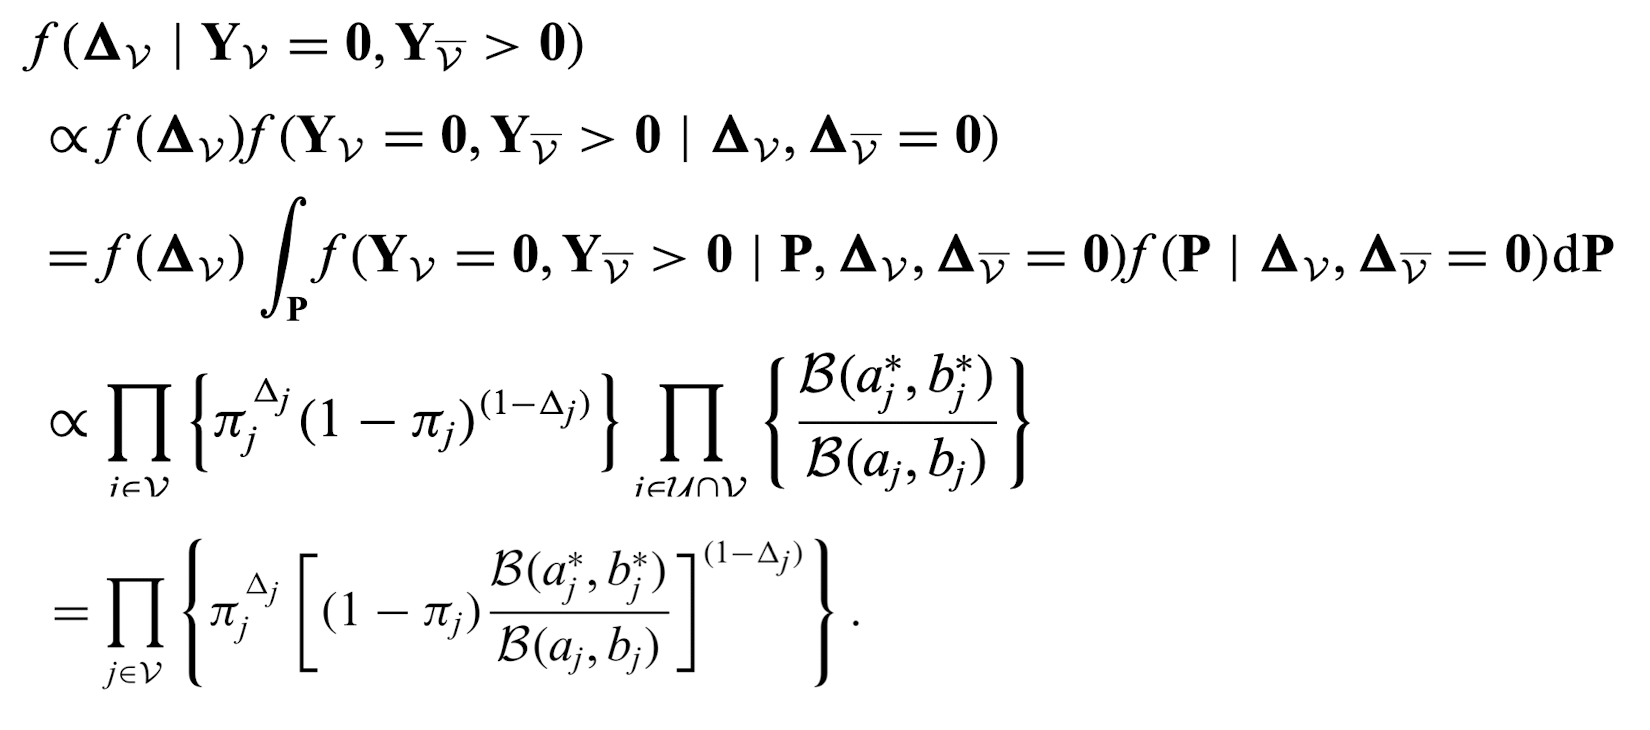
\includegraphics[width=0.95\textwidth]{img/2022.02.10_Zero_Inflated_generalized_Dirichlet_Multinomial-570dc718.png}
\end{figure}

\item Thus the posterior probability $f(\bm{P}|\bm{Y})$ follows a ZIGD with the zero-inflation on the taxa having observed zero counts
\item Probability of an observed zero being structural is
\begin{figure}[!htb]
	\centering
	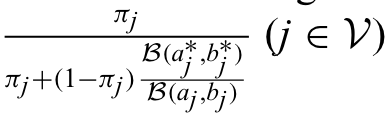
\includegraphics[width=0.35\textwidth]{img/2022.02.10_Zero_Inflated_generalized_Dirichlet_Multinomial-b0e76132.png}
\end{figure}
\end{itemize}
\end{frame}
%----------------------------------------------------------------------------------------

%----------------------------------------------------------------------------------------
\begin{frame}
\frametitle{ZIGDM Regression Model}
\begin{itemize}
  \item $n$ subjects measured on $K + 1$ taxa
  \item $Y_{ij}, P_{ij}$ observed count and true proportion for taxon $j$ in subject $i$.
  \item $\bm{X}_i$ $d$-dimensional vector of intercept, covariates, and confounding variables
  \item Assume $\bm{Y}_i$ follows a ZIGDM($\boldsymbol\pi_i, \bm{a}_i, \bm{b}_i$)
  \item The model is then
  \begin{figure}[!htb]
	\centering
	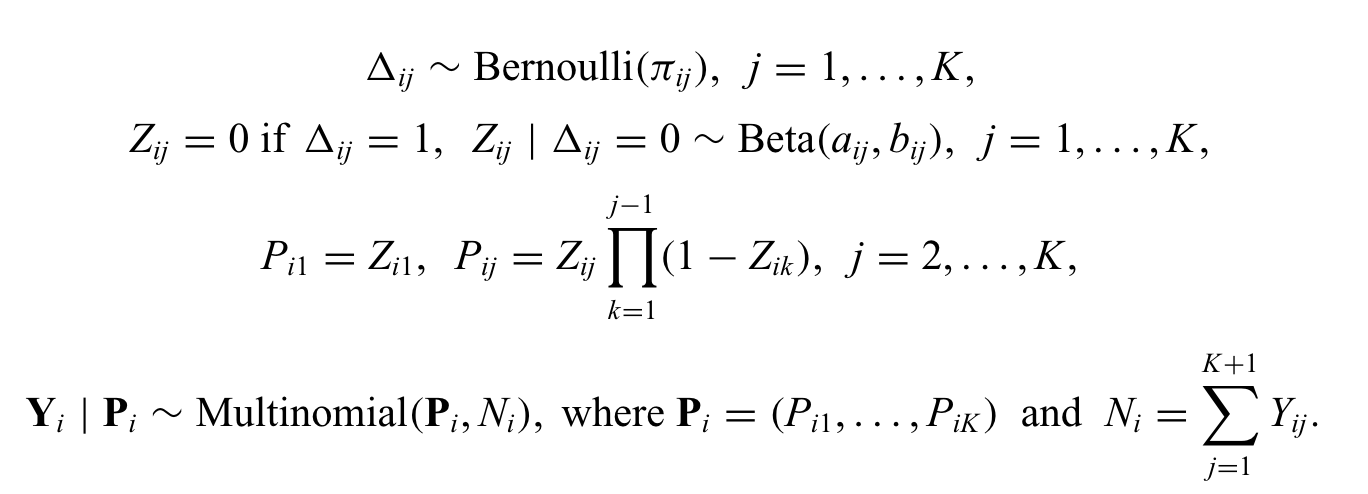
\includegraphics[width=0.95\textwidth]{img/2022.02.10_Zero_Inflated_generalized_Dirichlet_Multinomial-0ead4a93.png}
\end{figure}
\end{itemize}
\end{frame}
%----------------------------------------------------------------------------------------
%----------------------------------------------------------------------------------------
\begin{frame}
\frametitle{Link functions}
\begin{itemize}
  \item With this model, we can link $\boldsymbol\pi_i, \bm{a}_i,$ and $\bm{b}_i$ to $\bm{X}_i$
  \item $\pi_{ij}$ is the probability of absence % of taxon j in subject i
  \item $a_{ij}, b_{ij}$ control abundance distribution at the presence
  \item Reparametrize $\mu_{ij} = \frac{a_{ij}}{a_{ij} + b_{ij}}$ and $\sigma_{ij} = \frac{1}{1 + a_{ij} + b_{ij}}$ as the mean of the Beta variable and the dispersion parameter (since the variance of the Beta variables are of the form $\mu_{ij}(1 - \mu_{ij})\sigma_{ij}$)
  \item Use logit link functions ($\mu_{ij}, \mu_{ij}, \sigma_{ij}$ all between 0 and 1)
   \begin{figure}[!htb]
	\centering
	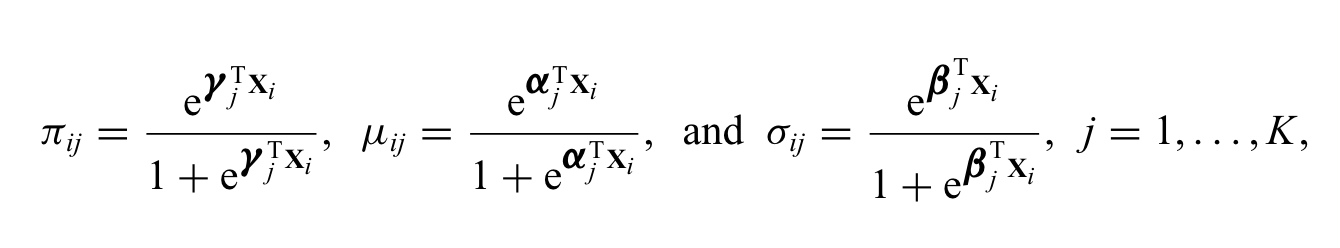
\includegraphics[width=0.75\textwidth]{img/2022.02.10_Zero_Inflated_generalized_Dirichlet_Multinomial-5360be17.png}
\end{figure}
\item $\boldsymbol\gamma_j = (\gamma_{1j}, \ldots, \gamma_{dj})$, $\boldsymbol\alpha_j = (\alpha_{1j}, \ldots , \alpha_{dj}), \boldsymbol\beta_j = (\beta_{1j}, \ldots , \beta_{dj})$ regression coefficients for taxon $j$.
\end{itemize}
\end{frame}
%----------------------------------------------------------------------------------------

%----------------------------------------------------------------------------------------
\begin{frame}
\frametitle{Estimating parameters}
\begin{itemize}
  \item Denote $\boldsymbol\theta = (\boldsymbol\gamma_1, \ldots , \boldsymbol\gamma_K, \boldsymbol\alpha_1, \ldots , \boldsymbol\alpha_K, \boldsymbol\beta_1, \ldots , \boldsymbol\beta_K)$ the complete set of parameters
  \item Likelihood-based inference on $\boldsymbol\theta$ is difficult since the observed log-likelihood function is complicated
  \item Complete data log-likelihood in terms of $Z$ (instead of $\bm P$)
  \begin{figure}[!htb]
	\centering
	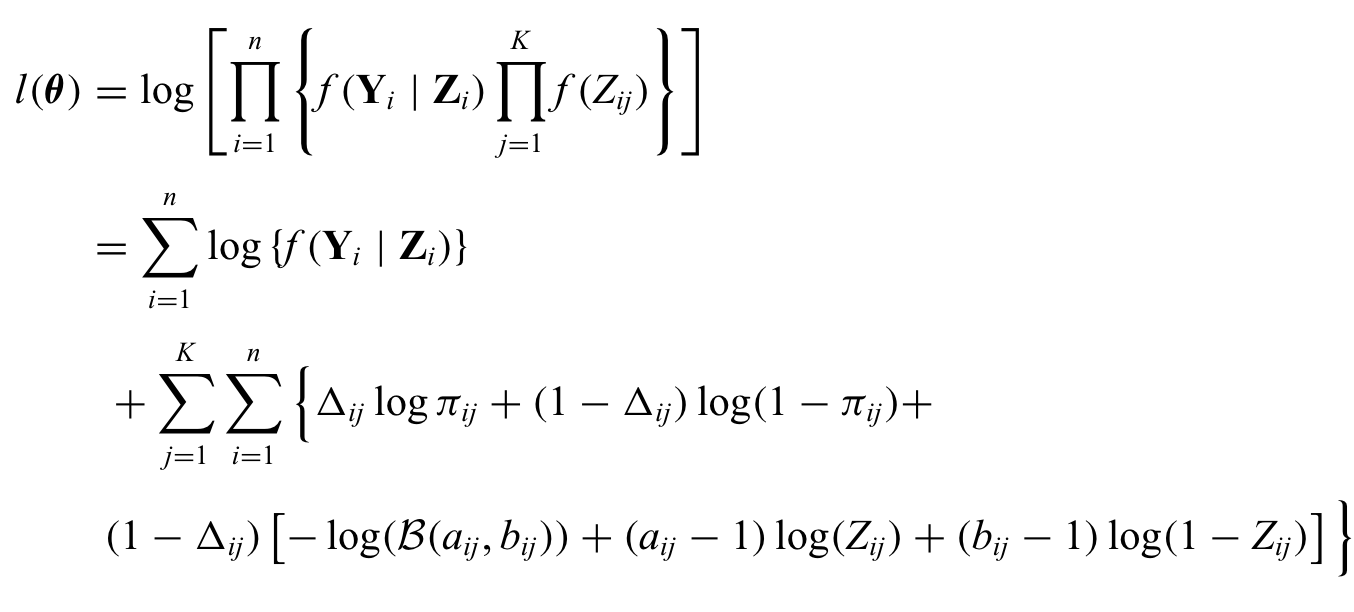
\includegraphics[width=0.95\textwidth]{img/2022.02.10_Zero_Inflated_generalized_Dirichlet_Multinomial-4c696321.png}
\end{figure}
\item $a_{ij} = \mu_{ij}(1/\sigma_{ij} - 1)$, $b_{ij} = (1 - \mu_{ij})(1/\sigma_{ij} - 1)$
\item Use $Z$ instead of $P$ to derive explicit form of the posterior expectations in the E-step and estimate parameters for each taxon independently in the M-step.
\end{itemize}
\end{frame}
%----------------------------------------------------------------------------------------

%----------------------------------------------------------------------------------------
\begin{frame}
\frametitle{EM algorithm for estimating parameters}
\begin{itemize}
  \item In the $t$-th E-step, compute the expected complete data log-likelihood:
  \begin{figure}[!htb]
	\centering
	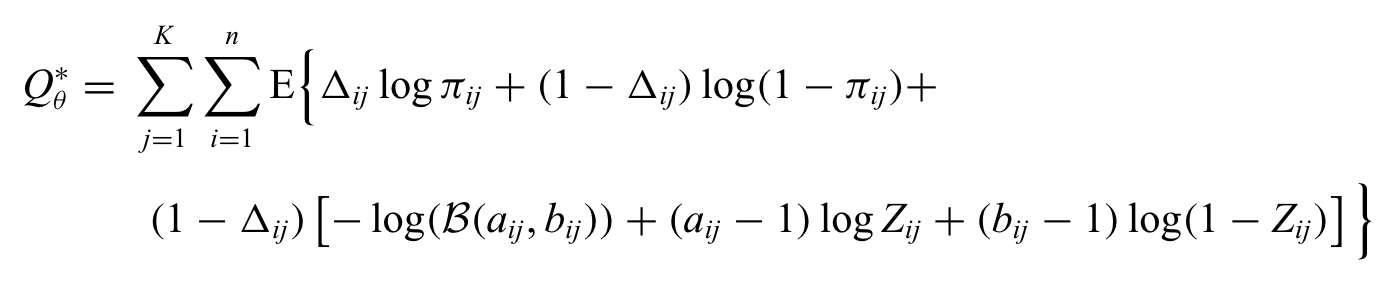
\includegraphics[width=0.95\textwidth]{img/2022.02.10_Zero_Inflated_generalized_Dirichlet_Multinomial-7ec4e475.png}
\end{figure}
\item Expectation is with respect to the posterior distributions of $(\boldsymbol\Delta_i| \bm{Y}_i; \boldsymbol\theta^{(t-1)})$ and $(\bm{Z}_i | \boldsymbol\Delta_i, \bm{Y}_i; \boldsymbol\theta^{t - 1})$
\item $\boldsymbol\theta^{(t-1)}$ the parameter estimates in the $(t -1)$-th M-step
\end{itemize}
\end{frame}
%----------------------------------------------------------------------------------------

%----------------------------------------------------------------------------------------
\begin{frame}
\frametitle{E - step}
\begin{itemize}
  \item
  \begin{figure}[!htb]
	\centering
	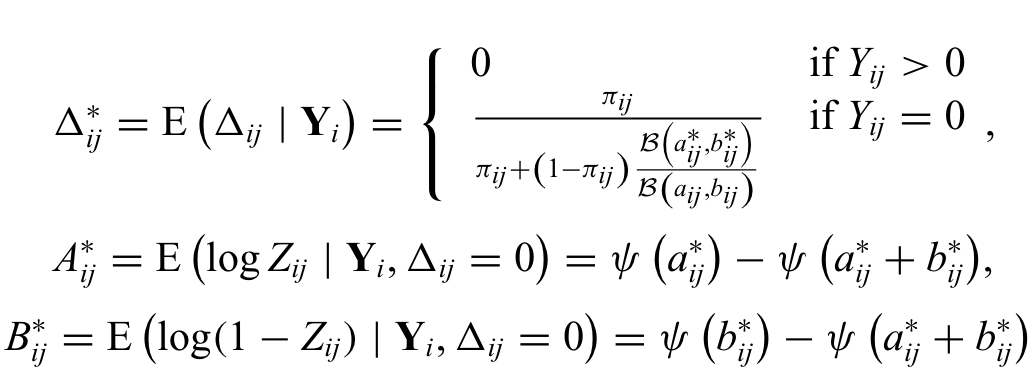
\includegraphics[width=0.75\textwidth]{img/2022.02.10_Zero_Inflated_generalized_Dirichlet_Multinomial-da36e885.png}
\end{figure}
\item $a_{ij}^* = a_{ij} + Y_{ij}, b_{ij}^* = b_{ij} + Y_{i(j+1)} + \cdots + Y_{i(K+1)}$, $\psi()$ is the digamma function
\item Rewrite $Q_\theta^*$ as:
 \begin{figure}[!htb]
	\centering
	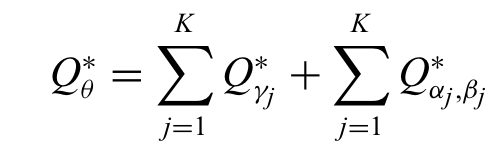
\includegraphics[width=0.35\textwidth]{img/2022.02.10_Zero_Inflated_generalized_Dirichlet_Multinomial-f8a319cd.png}
\end{figure}
\item $Q_{\gamma j}^* = \sum_{i=1}^n\{ \Delta_{ij}^* \log \pi_{ij} + (1 - \Delta_{ij}^*) \log(1 - \pi_{ij})\}$  and $Q_{\alpha_j, \beta_j}^* = \sum_{i=1}^n(1 - \Delta_{ij}^*)\{- \log (\mathcal{B}(a_{ij}, b_{ij})) + (a_{ij}-1)A_{ij}^* + (b_{ij} - 1)B_{ij}^*\}$
\end{itemize}
\end{frame}
%----------------------------------------------------------------------------------------

%----------------------------------------------------------------------------------------
\begin{frame}
\frametitle{M-Step}
\begin{itemize}
  \item In the $t$-th M-step, for each taxon $j$, obtain $\boldsymbol\gamma_j^{(t)}$ from maximizing $Q_{\gamma_j}^*$, and obtain $\boldsymbol\alpha_j^{(t)}, \boldsymbol\beta_{j}^{(t)}$ by maximizing $Q_{\alpha_j, \beta_j}^*$
  \item Computation for optimization is the same as a logisitic and weighted Beta regression
  \item Parameters for individual taxa updated independently, estimation can be done in parallel for different parameters
  \item Results in a computationally efficient EM algorithm relying on simple posterior estimation calculations and parallel parameter updates for taxa
\end{itemize}
\end{frame}
%----------------------------------------------------------------------------------------


%----------------------------------------------------------------------------------------
\begin{frame}
\frametitle{Association tests}
\begin{itemize}
  \item Test null hypothesis that covariates are not associated with the mean
$H_0: \bm{\alpha}_{*1} = \cdots = \bm{\alpha}_{*K} = 0$
\item Or covariates are not associated with dispersion
$H_0: \bm{\beta}_{*1} = \cdots = \bm{\beta}_{*K} = 0$
\item $\bm\alpha_{*j},\bm\beta_{*j}$ subsets of $\bm \alpha_j, \bm\beta_j$ corresponding to covariates of intersest

  \item Can test using score, Wald, or likelihood-ratio statistics
  \item This paper uses score statistics, which where computationally faster and more stable
  \item Use permutation techniques for $p$ values since asymptotic approximations may not be accurate when most observations are zero 
  \item Permute covariate of interest and calculate score test statistic in each permutation
\end{itemize}
\end{frame}
%----------------------------------------------------------------------------------------

%----------------------------------------------------------------------------------------
\begin{frame}
\Huge{\centerline{Thank you!}}
\end{frame}
%----------------------------------------------------------------------------------------

  \end{document}
